\documentclass[border=12pt]{standalone}
\usepackage{tikz}
\usetikzlibrary{arrows.meta, positioning, calc, fit, backgrounds}
\usepackage{amsmath}

\definecolor{frozen}{RGB}{180,210,240}
\definecolor{unfrozen}{RGB}{255,160,160}
\definecolor{newmod}{RGB}{255,220,130}
\definecolor{okgreen}{RGB}{170,230,170}
\definecolor{failred}{RGB}{255,180,180}
\definecolor{progblue}{RGB}{200,220,255}

\tikzset{
  B/.style={draw, rounded corners=3pt, minimum height=0.7cm, align=center, font=\footnotesize, thick, minimum width=2.8cm},
  F/.style={B, fill=frozen},
  U/.style={B, fill=unfrozen},
  N/.style={B, fill=newmod},
  OK/.style={B, fill=okgreen},
  a/.style={-{Stealth[length=2mm]}, thick},
  d/.style={-{Stealth[length=2mm]}, thick, dashed, red!60!black},
  tit/.style={font=\bfseries, align=center},
  res/.style={font=\scriptsize, align=center, rounded corners=3pt, draw, thick, inner sep=4pt, minimum width=3.2cm},
}

\begin{document}
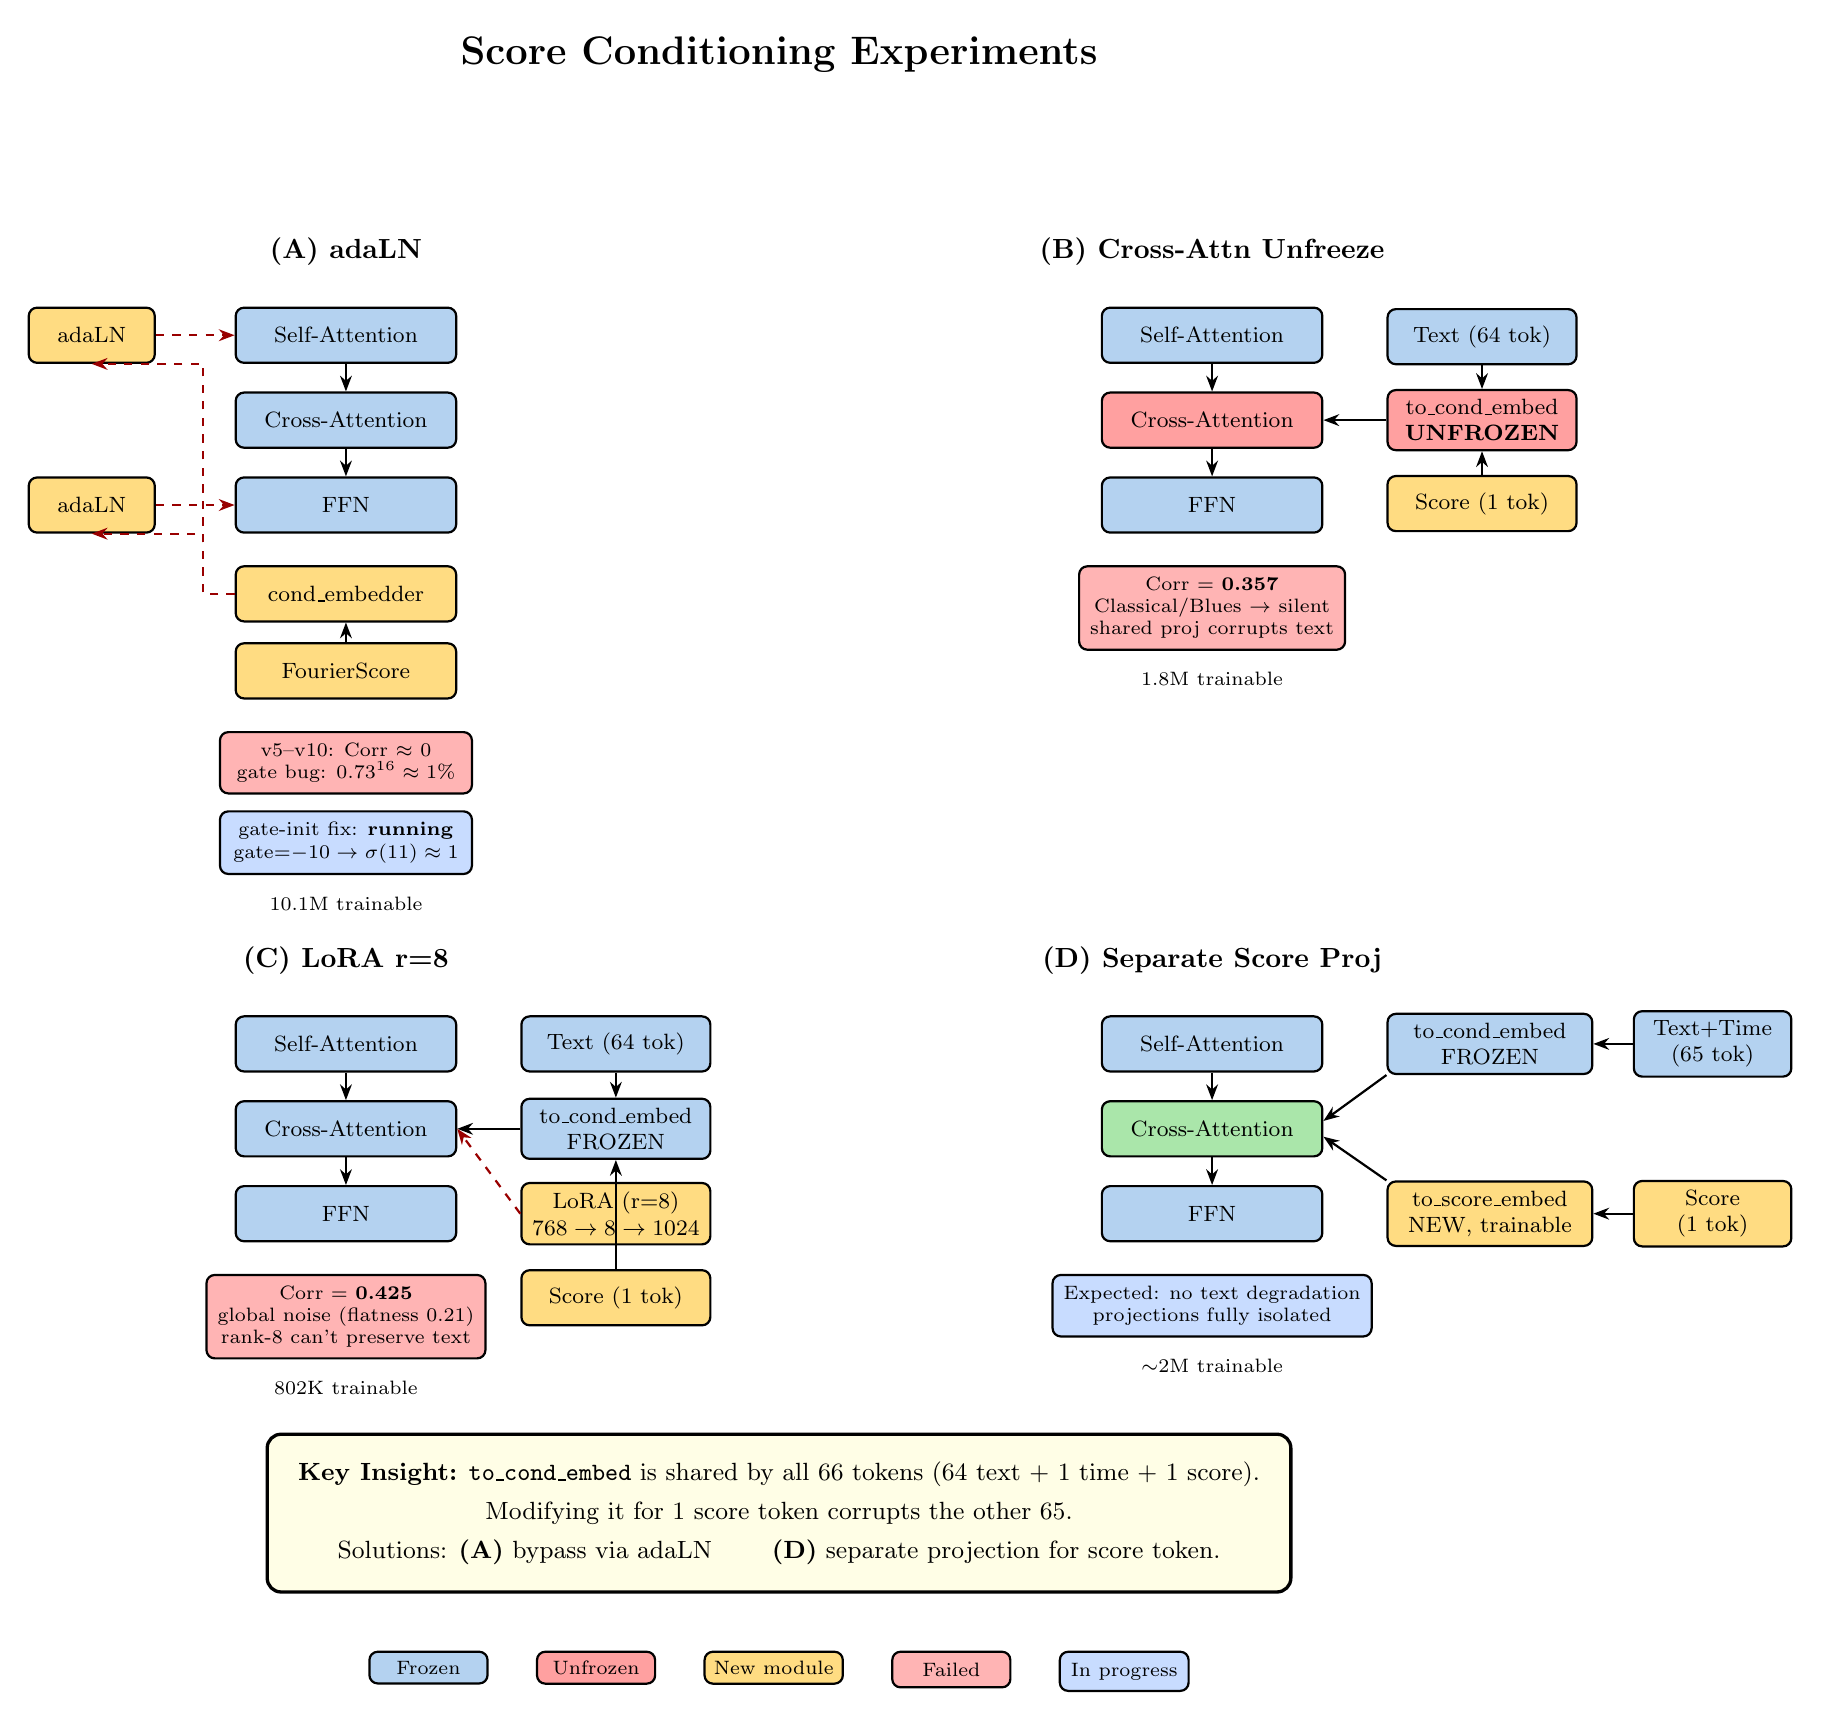
\begin{tikzpicture}

% ============================================================
% TITLE (centered)
% ============================================================
\node[font=\Large\bfseries, anchor=center] at (0,0) {Score Conditioning Experiments};

% ============================================================
% (A) adaLN — position (−5.5, −2)
% ============================================================
\begin{scope}[shift={(-5.5,-2.5)}]
  \node[tit, anchor=center] at (0,0) (tA) {(A) adaLN};

  \node[F, below=0.4cm of tA] (a1) {Self-Attention};
  \node[F, below=0.35cm of a1] (a2) {Cross-Attention};
  \node[F, below=0.35cm of a2] (a3) {FFN};
  \draw[a] (a1)--(a2);
  \draw[a] (a2)--(a3);

  % adaLN modules
  \node[N, left=1cm of a1, minimum width=1.6cm] (al1) {adaLN};
  \node[N, left=1cm of a3, minimum width=1.6cm] (al2) {adaLN};
  \draw[d] (al1)--(a1);
  \draw[d] (al2)--(a3);

  % Score path below
  \node[N, below=0.4cm of a3] (aemb) {cond\_embedder};
  \node[N, below=0.25cm of aemb] (asc) {FourierScore};
  \draw[a] (asc)--(aemb);
  \draw[d] (aemb.west) -- ++(-0.4,0) |- (al1.south);
  \draw[d] (aemb.west) -- ++(-0.4,0) |- (al2.south);

  % Results
  \node[res, fill=failred, below=0.4cm of asc] (ar1) {v5--v10: Corr $\approx$ 0\\gate bug: $0.73^{16} \approx 1\%$};
  \node[res, fill=progblue, below=0.2cm of ar1] (ar2) {gate-init fix: \textbf{running}\\gate=$-10 \to \sigma(11) \approx 1$};
  \node[font=\scriptsize, below=0.15cm of ar2] {10.1M trainable};
\end{scope}

% ============================================================
% (B) Cross-Attn Unfreeze — position (+5.5, −2)
% ============================================================
\begin{scope}[shift={(5.5,-2.5)}]
  \node[tit, anchor=center] at (0,0) (tB) {(B) Cross-Attn Unfreeze};

  \node[F, below=0.4cm of tB] (b1) {Self-Attention};
  \node[U, below=0.35cm of b1] (b2) {Cross-Attention};
  \node[F, below=0.35cm of b2] (b3) {FFN};
  \draw[a] (b1)--(b2);
  \draw[a] (b2)--(b3);

  % Conditioning (right)
  \node[U, right=0.8cm of b2, minimum width=2.4cm] (btc) {to\_cond\_embed\\\textbf{UNFROZEN}};
  \node[F, above=0.3cm of btc, minimum width=2.4cm] (btxt) {Text (64 tok)};
  \node[N, below=0.3cm of btc, minimum width=2.4cm] (bsc) {Score (1 tok)};
  \draw[a] (btxt)--(btc);
  \draw[a] (bsc)--(btc);
  \draw[a] (btc)--(b2);

  % Results
  \node[res, fill=failred, below=0.4cm of b3] (br) {Corr = \textbf{0.357}\\Classical/Blues $\to$ silent\\shared proj corrupts text};
  \node[font=\scriptsize, below=0.15cm of br] {1.8M trainable};
\end{scope}

% ============================================================
% (C) LoRA — position (−5.5, −11)
% ============================================================
\begin{scope}[shift={(-5.5,-11.5)}]
  \node[tit, anchor=center] at (0,0) (tC) {(C) LoRA r=8};

  \node[F, below=0.4cm of tC] (c1) {Self-Attention};
  \node[F, below=0.35cm of c1] (c2) {Cross-Attention};
  \node[F, below=0.35cm of c2] (c3) {FFN};
  \draw[a] (c1)--(c2);
  \draw[a] (c2)--(c3);

  % Conditioning (right, stacked cleanly)
  \node[F, right=0.8cm of c1, minimum width=2.4cm] (ctxt) {Text (64 tok)};
  \node[F, right=0.8cm of c2, minimum width=2.4cm] (ctc) {to\_cond\_embed\\FROZEN};
  \node[N, right=0.8cm of c3, minimum width=2.4cm] (clora) {LoRA (r=8)\\$768 \to 8 \to 1024$};
  \node[N, below=0.3cm of clora, minimum width=2.4cm] (csc) {Score (1 tok)};

  \draw[a] (ctxt)--(ctc);
  \draw[a] (csc)--(ctc);
  \draw[a] (ctc)--(c2);
  % LoRA adds residual to projection output
  \draw[d] (clora.west) -- (c2.east);

  % Results
  \node[res, fill=failred, below=0.4cm of c3] (cr) {Corr = \textbf{0.425}\\global noise (flatness 0.21)\\rank-8 can't preserve text};
  \node[font=\scriptsize, below=0.15cm of cr] {802K trainable};
\end{scope}

% ============================================================
% (D) Separate Score Proj — position (+5.5, −11)
% ============================================================
\begin{scope}[shift={(5.5,-11.5)}]
  \node[tit, anchor=center] at (0,0) (tD) {(D) Separate Score Proj};

  \node[F, below=0.4cm of tD] (d1) {Self-Attention};
  \node[OK, below=0.35cm of d1] (d2) {Cross-Attention};
  \node[F, below=0.35cm of d2] (d3) {FFN};
  \draw[a] (d1)--(d2);
  \draw[a] (d2)--(d3);

  % Two separate projections (right, stacked)
  \node[F, right=0.8cm of d1, minimum width=2.6cm] (dtc) {to\_cond\_embed\\FROZEN};
  \node[F, right=0.5cm of dtc, minimum width=2cm] (dtxt) {Text+Time\\(65 tok)};
  \draw[a] (dtxt)--(dtc);
  \draw[a] (dtc.south west) -- ($(d2.east)+(0,0.1)$);

  \node[N, right=0.8cm of d3, minimum width=2.6cm] (dts) {to\_score\_embed\\NEW, trainable};
  \node[N, right=0.5cm of dts, minimum width=2cm] (dsc) {Score\\(1 tok)};
  \draw[a] (dsc)--(dts);
  \draw[a] (dts.north west) -- ($(d2.east)+(0,-0.1)$);

  % Results
  \node[res, fill=progblue, below=0.4cm of d3] (dr) {Expected: no text degradation\\projections fully isolated};
  \node[font=\scriptsize, below=0.15cm of dr] {$\sim$2M trainable};
\end{scope}

% ============================================================
% Key Insight box (centered below all)
% ============================================================
\node[draw, very thick, rounded corners=5pt, fill=yellow!10,
      minimum width=13cm, align=center, inner sep=10pt, font=\small,
      anchor=north] at (0,-17.5) (insight) {
\textbf{Key Insight:} \texttt{to\_cond\_embed} is shared by all 66 tokens (64 text + 1 time + 1 score).\\[3pt]
Modifying it for 1 score token corrupts the other 65.\\[3pt]
Solutions: \textbf{(A)} bypass via adaLN \qquad \textbf{(D)} separate projection for score token.
};

% ============================================================
% Legend (centered below insight)
% ============================================================
\matrix[anchor=north, below=0.6cm of insight, column sep=0.6cm] {
  \node[F, minimum width=1.5cm, minimum height=0.35cm, font=\scriptsize]{Frozen}; &
  \node[U, minimum width=1.5cm, minimum height=0.35cm, font=\scriptsize]{Unfrozen}; &
  \node[N, minimum width=1.5cm, minimum height=0.35cm, font=\scriptsize]{New module}; &
  \node[res, fill=failred, minimum width=1.5cm, font=\scriptsize]{Failed}; &
  \node[res, fill=progblue, minimum width=1.5cm, font=\scriptsize]{In progress}; \\
};

\end{tikzpicture}
\end{document}
